\documentclass[12pt]{article}
\usepackage[paper=letterpaper,margin=2cm]{geometry}
\usepackage{amsmath}
\usepackage{amssymb}
\usepackage{amsfonts}
\usepackage{newtxtext, newtxmath}
\usepackage{enumitem}
\usepackage{titling}
\usepackage[colorlinks=true]{hyperref}
\usepackage{graphicx}
\usepackage{float}
\usepackage{listings}
\usepackage{xcolor}
\usepackage{color}
\definecolor{dkgreen}{rgb}{0,0.6,0}
\definecolor{gray}{rgb}{0.5,0.5,0.5}
\definecolor{mauve}{rgb}{0.58,0,0.82}
\lstset{ %
        language=Java,                
  basicstyle=\footnotesize,     
  numbers=left,               
  numberstyle=\tiny\color{gray},
  stepnumber=1,                                       
  numbersep=5pt,                 
  backgroundcolor=\color{white},  
  showspaces=false,             
  showstringspaces=false,         
  showtabs=false,                 
  frame=single,                   
  rulecolor=\color{black},       
  tabsize=4,                   
  captionpos=b,        
  breaklines=true,             
  breakatwhitespace=false,       
  title=\lstname,                                                  
  keywordstyle=\color{blue},          
  commentstyle=\color{dkgreen},    
  stringstyle=\color{mauve},       
  escapeinside={\%*}{*},        
  morekeywords={*,...}
} 

\setlength{\droptitle}{-6em}

% Enter the specific assignment number and topic of that assignment below, and replace "Your Name" with your actual name.
\title{Assignment 2: Comp 6771 Image Processing}
\author{Yunqi Xu 40130514}
\date{\today}



\begin{document}
% \maketitle

\begin{titlepage}
  \rule{\textwidth}{1pt}   % The top horizontal rule
    \vspace{0.2\textheight}  % Whitespace between top horizontal rule and title

    %------------------------------------------------------------
    %    Title
    %------------------------------------------------------------

    {\Huge COMP 6771 Image Processing: Assignment 2}

    \vspace{0.025\textheight}   % Whitespace between the title and short horizontal rule

    \rule{0.83\textwidth}{0.4pt}  % The short horizontal rule under title

    \vspace{0.1\textheight}  % Whitespace between the short horizontal rule and author

    %------------------------------------------------------------
    %    Author
    %------------------------------------------------------------

    {\Large Student name: \textsc{Yunqi Xu}}
    \vfill
    {\Large Student id: 40130514}
    \vfill  % Whitespace between author and date

    {\large \today}
    \vspace{0.1\textheight}  % Whitespace between date and bottom horizontal rule

    %------------------------------------------------------------
    %    Bottom rules
    %------------------------------------------------------------

    \rule{\textwidth}{1pt}  % The bottom horizontal rule
\end{titlepage}

\begin{enumerate}[leftmargin=\labelsep]
% \vspace*{40em}
\item Question 1
    \begin{enumerate}
    \item The minimum size of the blur mask is a 7 * 7 filter.
    Since the averaging filter will calculate the average of the pixels contined in the neighborhood of the filter mask. 
    No matter the coefficient value off the average filter is. 
    If all pixels in the filter mask are zero, the output is zero. 
    Based on the question, the gaps ranging from 1 to 5 pixels. 
    So the minimum kernal size should greater than 5 to avoid the zero output.
    Also, the kernel size usually is odd number.
    So, 7 * 7 is the minimum size.

    \vspace*{1em}

    
    \item Based on the question, we want those ouput which the filter center located on the string or hole(and be filled) equal or greater than the threshold and keep those value.
    Suppose the center of the filter located at a center of a gap. 
    In this case, the filter will have a minimum output that we want to convert it value. 
    Also, the maximum size of gap is 5 pixels.  
    If we want to use thresholding method to convert it back at the meanwhile keep string without small hole or noise, we need to guarantee that the minimum ouput greater than threshold.
    So, suppose we get S as the minumum useful output.
    We will set threshold closely less than S, but not less too much. 
    To do this, we can keep string without small hole and abvoid to bring more noise during the threshold process.
    \vspace*{1em}


    \end{enumerate}

\item Question 2

The 5-by-5 Laplacian like filter has been shown in Eq.~\ref{q2_eq1} below: 

\begin{equation}
\begin{bmatrix}
        0 & 0 & 1   & 0 & 0 \\
        0 & 1 & 2   & 1 & 0 \\
        1 & 2 & -16 & 2 & 1 \\
        0 & 1 & 2   & 1 & 0 \\
        0 & 0 & 1   & 0 & 0 
\end{bmatrix}
\label{q2_eq1}
\end{equation}

The basic rule is the sum of all coefficient is 0.

We will use $g(x, y) = f(x,y) - \bigtriangledown^2 f(x,y) $ to sharpen an image.
Compared with filters in question, this one will output an image sharper result.
Because, the center of the 5-by-5 filters have more weight than $-4$ or $-8$.
So, the edge of the image will be further enhence.

\vspace*{1em}

\item Question2 Fourier Transform Queston
\begin{enumerate}
        \item Based on the question, the Eq.~\ref{q2_eq2} defines the variable t.
        \begin{equation}
                f(t) =
                \begin{cases}
                A & 0 \leq t \leq W \\
                0 & otherwase 
                \end{cases}   
        \label{q2_eq2}    
        \end{equation}
        

        \begin{equation}
        \begin{aligned}
        F(\mu)
        &= \int_{-\infty}^{+\infty}f(t) e^{-j2 \pi \mu t}dt\\
        &= \int_0^W A e^{-j2 \pi \mu t} dt\\
        &= \frac{-A}{j2 \pi \mu} [e^{-j 2 \pi \mu t}]_{0}^{W}\\
        &= \frac{-A}{j2 \pi \mu} [e^{-j 2 \pi \mu W}  - 1]\\
        &= \frac{A}{j2 \pi \mu} [1 - e^{-j2 \pi \mu W}]\\
        &= \frac{A}{j2 \pi \mu} [e^{j \pi \mu W - e^{-j \pi \mu W}}]e^{-j \pi \mu W}\\
        &= AW (\frac{sin(\pi \mu W)}{\pi \mu W}) e^{-j \pi \mu W}
        \label{q2_eq3}
        \end{aligned}
        \end{equation}
        Since $A = W = 1 $, In the Example, the result is:
        \begin{equation}
            F(\mu) = AW \frac{sin(\pi \mu W)}{\pi \mu W} = \frac{sin(\pi \mu)}{\pi \mu}
        \label{q2_eq4}
        \end{equation}
        And the result of Eq.~\ref{q2_eq3} is:
        \begin{equation}
            F(\mu) = \frac{sin(\pi \mu)}{\pi \mu} e^{-j \pi \mu}
        \label{q2_eq5}
        \end{equation}
        Compared with these two equation Eq.~\ref{q2_eq4} and Eq.~\ref{q2_eq5}, the only different part is $e^{-j \pi \mu}$. So the case in this problem is a shifted part compared the resul of Example 4.1.
        \vspace*{1em}
        \item   
        Based on the property of Convolution:
        $$
            f(t) \star h(t) \Longleftrightarrow H(\mu)F(\mu)
        $$
        
        \begin{equation}
        f(t) =
        \begin{cases}
        A & \frac{-W}{2} \leq t \leq \frac{W}{2} \\
        0 & otherwase 
        \end{cases}   
        \label{q2_eq6}    
        \end{equation}
        Based on the information provided by the right image in question, the Eq.~\ref{q2_eq6} is the equation.

        \begin{equation}
        \begin{aligned}
        F(\mu)
        &= \int_{-\infty}^{+\infty}f(t) e^{-j2 \pi \mu t}dt\\
        &= \int_{\frac{-W}{2}}^{\frac{W}{2}} A e^{-j2 \pi \mu t} dt\\
        &= \frac{-A}{j2 \pi \mu} [e^{-j 2 \pi \mu t}]_{\frac{-W}{2}}^{\frac{W}{2}}\\
        &= AW (\frac{sin(\pi \mu W)}{\pi \mu W})
        \label{q2_eq7}
        \end{aligned}
        \end{equation}

        Based on the property of convolution and Eq.~\ref{q2_eq7}, the Fourier Transform of the tent function is: 
        \begin{equation}
        \begin{aligned}
        F(\mu)F(\mu)
        &= A^2 W^2 \frac{sin^2(\pi \mu W)}{\pi^2 \mu^2 W^2}\\
        &= A^2 \frac{sin^2(\pi \mu W)}{\pi^2 \mu^2}
        \label{q2_eq8}
        \end{aligned}
        \end{equation}


        \vspace*{1em}
        
\end{enumerate}

\item Question 3.
\begin{enumerate}
\item The code has been shown below

\begin{lstlisting}
import numpy as np
import cv2


# read image
def readimg(path):
    return cv2.imread(path, 0)

# Generate a Gaussian filter
def GaussinFilter(sigma, size):
    m = (size - 1.) / 2.
    n = (size - 1.) / 2.
    y, x = np.ogrid[-m:m + 1, -n: n + 1]
    h = np.exp(-(x * x + y * y) / (2. * sigma * sigma))
    h[h < np.finfo(h.dtype).eps * h.max()] = 0
    all_sum = h.sum()
    if all_sum != 0:
        h /= all_sum
    return h



# Using gaussian to get the weighted aaverage.
def weightedSum(input_subimage, input_filter, filter_size):
    new_subimage = np.zeros((filter_size, filter_size))
    for y in range(filter_size):
        for x in range(filter_size):
            new_subimage[y, x] = input_subimage[y, x] * input_filter[y, x]
    return sum(sum(new_subimage))


def averagingFilter(input_image, input_filter, filter_size):
    image_height, image_width = input_image.shape[0], input_image.shape[1]
    output_image = np.zeros((image_height,image_width))
    padding_size = int((filter_size - 1) / 2)
    padding_short = np.zeros((padding_size, image_width))
    padding_long = np.zeros((image_height + (filter_size - 1), padding_size))
    padded_image = np.r_[padding_short, input_image]
    padded_image = np.r_[padded_image, padding_short]
    padded_image = np.c_[padding_long, padded_image]
    padded_image = np.c_[padded_image, padding_long]

    for y in range(padding_size, image_height + padding_size):
        for x in range(padding_size, image_width + padding_size):
            sub_image = padded_image[y - padding_size: y + (padding_size + 1), x - padding_size: x + (padding_size + 1)]
            output_image[y - padding_size, x - padding_size] = weightedSum(
                                        input_subimage=sub_image, 
                                        input_filter=input_filter, 
                                        filter_size=filter_size)
    return output_image



def calculateThreshold(input_image, C):
    image_height, image_width = input_image.shape
    output_image = np.zeros((image_height,image_width))
    for y in range(image_height):
        for x in range(image_width):
            output_image[y, x] = input_image[y, x] - C
    return output_image


# threshold the image
def threshold(input_image, max_value, threshold):
    output_image = np.zeros((input_image.shape[0], input_image.shape[1]))
    height, width = input_image.shape
    for y in range(height):
        for x in range(width):
            if input_image[y, x] >= threshold[y, x]:
                output_image[y, x] = max_value
            else:
                output_image[y, x] = 0
    return output_image


# The overall Adaptive thresholding
def adaptiveThresholding(input_image, 
        max_value, adaptive_method, 
                threshold_type, filter_size,
                 C, Gaussian_sigma=1.4):
    if adaptive_method == "Gaussian":
        filter = GaussinFilter(sigma=Gaussian_sigma,
                         size=filter_size)

    wa_image = averagingFilter(input_image=input_image, input_filter=filter, filter_size=filter_size)


    if threshold_type == "THRESH_BINARY":
        t_image = calculateThreshold(input_image=wa_image, C=C)

    threshold_image = threshold(input_image=input_image, max_value=max_value, threshold=t_image)

    output_image = np.array(threshold_image, dtype='uint8')

    return output_image



image = readimg("Doc.tiff")
output_image = adaptiveThresholding(
        input_image=image, 
        max_value=255, 
        adaptive_method="Gaussian",         
        threshold_type="THRESH_BINARY", 
        filter_size=11, 
        C = 4.5, 
        Gaussian_sigma=3)
cv2.imwrite('output.png', output_image)
\end{lstlisting}

\item In this question, we choose the Gaussian filter as the coefficient when calculateng the weighted average. The reason is that, Mean filter is good at reducing random noise, but in our image, we want to split the foreground and background. And Gaussian filter can achieve a better result compared with Mean filter when dealing with the problem of spliting two different frequencies.

Also, The filter\_size we choose is 11, since the letter in image are around 11 pixels for each of them. and the Gaussian\_sigma = 3. Usualy, a higher gussian sigma will get a gaussian filter that can bring more neighborhood inforamtion to the center.

\begin{figure}[H]
        \centering
        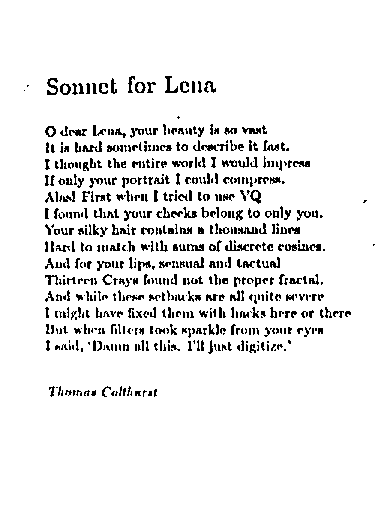
\includegraphics[]{Figure/output.png}
        \caption{The output image of Python implement}
        \label{Q3_1}
\end{figure}

\begin{figure}[H]
        \centering
        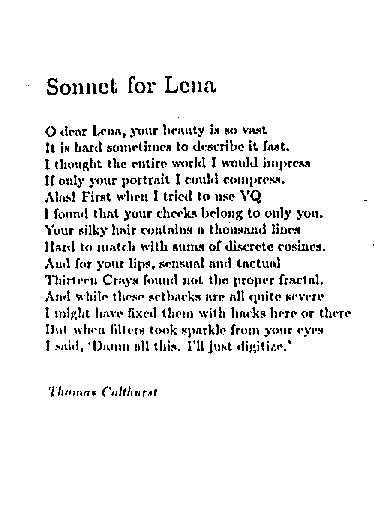
\includegraphics[]{Figure/cv2_output.png}
        \caption{The output image from open cv2.adaptiveThreshold}
        \label{Q3_2}
\end{figure}

\begin{figure}[H]
        \centering
        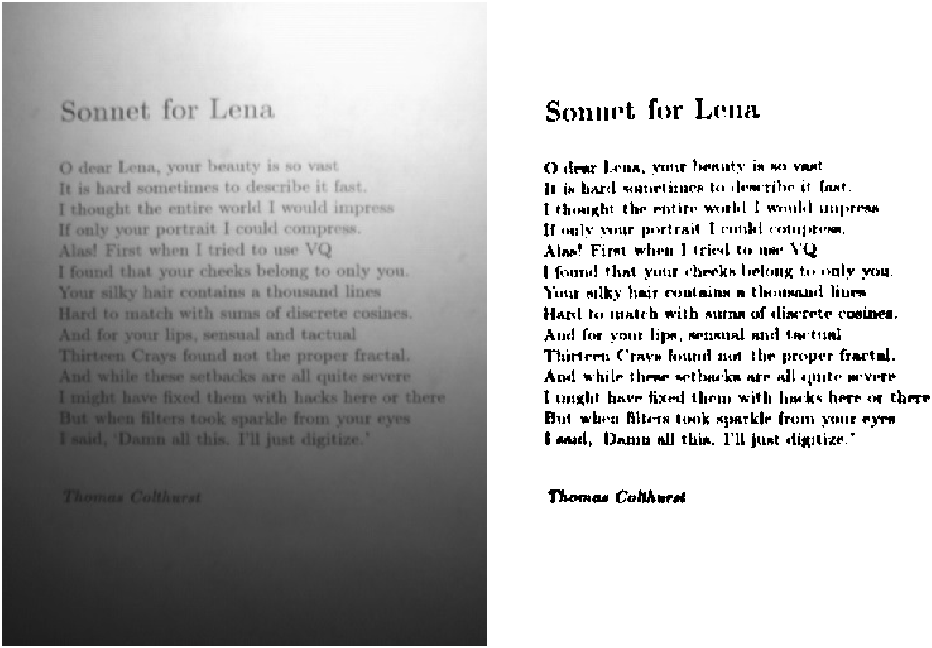
\includegraphics[]{Figure/A2mo.png}
        \caption{The output image from Matlab adaptthresh}
        \label{Q3_3}
\end{figure}

The Fig.~\ref{Q3_1} is the output by using the code above. And the Fig.~\ref{Q3_2} is the output from the method which is provided by OpenCV cv2.adaptiveThreshold() and we use the same parameters as we used in the implemented code. The Fig.~\ref{Q3_3} is the output image from the Matlab adaptthresh() with the same parameters. All of these three function can separate the input image from the dark backgroud. The implemented code and the function from openCV can achieve a slightly better result may because there are more parameters that could be modified such as the sigma of gaussian. 

\end{enumerate}



\end{enumerate}

\end{document}
